\documentclass{jsarticle}
\usepackage{color}
\usepackage{bm}
 \usepackage[height=26cm,width=16cm]{geometry} 
 \usepackage{amsmath}
 \usepackage{cases}
\usepackage[dvipdfmx]{graphicx}
\graphicspath{{./image/}}

\title{数理計画}

\begin{document}

\maketitle

\section{10/29}
\section{数理計画}
	最適化すべき問題を数学モデルに定式化し、それを解く\\
		{\Large{目的}}\\
		1.様々な問題を数学モデルに定式化できること\\
		2.シンプレックス法を用いて、線形計画問題を解けること\\
	※この二つをテストで確かめられる\\
	※線形計画も線形って何?テストに出るよ

\section{1章  数理計画モデル}
{\Large{目的}}\\
	1.数理計画法の考え方を知る\\
	2.数理計画問題を定式化する\\
		\subsection{線形計画モデル}
			\subsubsection{生産計画問題}
				たぶん、教科書に書いてある4種類の原料A,B,C,Dを用いるやつ。それぞれ80,50,100,70のやつ\\
				目的 : 最大の利益をあげたい↓\\
				\[
					70x_1+120x_2+30x_3\\
				\]
				これを{\large{目的関数}}という\\
				この利益を最大にしたい\\
				目的関数:$70x_1+120x_2+30x_3→Max$\\
				核原料には使用量に制約がある\\
				原料Aは80単位まで使える\\
				\[
					5x_1    +6x_3≦80
				\]
				同様に
				\begin{eqnarray}
					      2x_2+8x_3≦50\\
					70x_1     +15x_3≦100\\
					3x_1+11x_2     ≦70\\
				\end{eqnarray}
				定式化\\
				目的関数:\[70x_1+120x_2+30x_3→Max\]
				制約条件:\\
				\begin{eqnarray}
					5x_1    +6x_3≦80\\
					      2x_2+8x_3≦50\\
					70x_1     +15x_3≦100\\
					3x_1+11x_2     ≦70\\
					x_1≧0,x_2≧0,x_3≧0 &→ 非負条件\\
				\end{eqnarray}
				生産計画問題は\\
				制約条件のもとで、目的関数が最大となる変数$x_1,x_2,x_3$の値を求める問題に定式化できる\\
				{\Large{線形計画問題とは・・・}}\\
				制約条件が1次の等式や不等式で表され、かつ、目的関数が1次関数である問題のことである\\
				\subsubsection{多期間計画問題}
					t月における製品$i=1,2$の生産量を$x_{it}$とし、t月から翌月に持ち越す在庫量を$y_{it}$とする\\
					{\textcolor{red}{コストを最小化したい!}\\
					3ヶ月間の総コストを考える\\
					目的関数:\\
					\begin{eqnarray}
						75(x_{11}+x_{12}+x_{13})+50(x_{21}+x_{22}+x_{23}) &→生産コスト\\ 
						+8(y_{11}+y_{12})+7(y_{21}+y_{22}) &→在庫コスト\\
						→最小
					\end{eqnarray}
					制約条件\\
					原料の利用可能量(上限)
					A:\\
					1月:$2x_{11}+7x_{21}≦920$\\
					2月:$2x_{12}+7x_{22}≦750$\\
					3月:$2x_{13}+7x_{23}≦500$\\
					B:\\
					1月;$5x_{11}+3x_{12}≦790$\\
					2月:$5x_{12}+3x_{22}≦600$\\
					3月:$5x_{13}+3x_{23}≦480$\\
					(実際のテストの時にはAとかBとか1月とか書かなくていい)\\
					出荷量に関する制約\\
					I:\\
					1月:$x_{11}-y_{11}=30$\\
					2月:$x_{12}+y_{11}-y_{12}=60 前の在庫もたす$\\
					3月:$x_{13}+y_{12}=80 在庫いらない$\\
					II:\\
					1月:$x_{21}-y_{21}=20$\\
					2月:$x_{22}+y_{21}-y_{22}=50$\\
					3月:$x_{23}-y_{22}$\\
					非負条件は\\
					$x_{it}≧0 , i=1,2 ,t=1,2,3$\\
					$y_{it}≧0, i=1,2 , t=1,2$\\
			\subsubsection{輸送計画問題}
				工場$A_i(i=1,2,3)$から取引先$B_j(j=1,2,3)$への輸送量を$x_{ij}$で表す\\
				{\textcolor{blue}{輸送コスト}\\
				目的関数:\\
				\begin{eqnarray}
					4_x{11}+7_x{12}+12x_{13}+11x_{21}+6x_{22}+3x_{23}→最小
				\end{eqnarray}
				制約条件:\\
					生産量\\
					$A_1$:$x_{11}+x_{12}+x_{13}=90$\\
					$A_2$:$x_{21}+x_{22}+x_{23}=80$\\
					注文に関数制約\\
					$B_1$:$x_{11}+x_{21}=70$\\
					$B_2$ : $x_{12}+x_{22}=40$\\
					$B_3$ : $x_{13}+x_{23}=60$\\
					非負条件\\
					$x_{ij}≧0 , i=1,2 , j=1,2,3$\\
					
\section{11/5}
\section{ネットワークモデル}
	グラフ;いくつかの点とそれらを結ぶ矢印からなる\\
	いくつかの点→節点(ノード)、結ぶ矢印→枝(アーク)\\
	有向グラフ:枝に向きがある\\
	無向グラフ:枝に向きがない\\
	節点iからjへの枝を$(i,j)$で表す\\
	例→教科書\\

	節点$V=\{1,2,3,4\}$→ここは絶対中括弧\\
	枝全体の集合\\
	$E={(1,2),(1,3),(2,4),(3,2),(3,4),(4,2)}$\\
	グラフ$G=(V,E)$\\
	で表す\\
	節点1から節点4への路(パス)\\
	$P={(1,2,4),(1,3,4),(1,3,2,4)}$\\
	路$P=(1,2,4)$への長さ\\
	枝$(i,j)$を通るかどうかを変数にとる\\
	$x=$
	\begin{numcases}
			1 & (i,j)を通る\\
			0 & (i,j)を通らない\\
	\end{numcases}\\
	→0-1条件
	目的関数→総所要時間\\
	\[
		\sum_{(i,j)∈E}a_{ij}x_{ij}=5x_{AB}+4x_{AC}+2x_{BC}+4x_{BD}+7x_{BE}+2x_{CB}+6x_{CD}+8x_{CF}+5x_{DE}+3x_{DF}+x_{EF}+3x_{EG}+2x_{FE}+2x_{FG}→最小
	\]
	制約条件\\
	A→$-x_{AB}-x_{AC}=-1$\\
	B→$x_{AB}+x_{CB}-x_{BC}-x_{BD}-x_{BE}=0$\\
	C→$x_{AC}+x_{BC}-x_{CB}-x_{CD}-x_{CF}=0$\\
	D→\\
	E\\
	F\\
	G\\
	\subsection{最大流問題}
		教科書みてね\\
		定式化\\
		枝$(i,j)$の輸送量を$x_{ij}$とおく\\
		各枝の容量を$u_{ij}$で表す \\
		際流量(輸送できる最大値)をfとおく\\
		目的関数:f→最大\\
		制約条件:→教科書\\
		容量制約条件\\
		$0≦x_{ij}≦u_{ij} , (i,j)∈E$
	
	\subsection{資源配分問題}
		定式化\\
		各科目の勉強時間を$t_1,t_2,t_3$時間とおく→何を何でおいたかは必ず書く\\
		目的関数:$h_1(t_1)+h_2(t_2)+h_3(t_3)$→最大\\
		制約関数:\\
		\begin{equation}
			t_1+t_2+t_3=T\\
			t_i≧0,i=1,2,3\\
		\end{equation}
		
	\subsection{ポートフォリオ選択問題}
		各株式への投資額を$x_1,x_2,x_3$円とする\\
		1ヶ月後の予想株価を$q_1,q_2,q_3$円とおく\\
		各株式に何口投資したか\\
		利益\\
		\begin{equation}
			z=W-w\\
			=\frac{x_1}{P_1}q_1+\frac{x_2}{P_2}q_2+\frac{x_3}{P_3}q_3-(x_1+x_2+x_3)\\
			=R_1x_1+R_2x_2+R_3x_3\\
			R_i=\frac{q_i-P_i}{P_i}とおく\\
		\end{equation}
		これを収益率という

\section{11/19}
	\subsection{交通流割り当て問題}
	(教科書参照)図のような道路網を考える。道路管理者が道路網の効率利用の点から交通流を調整する時、どのようにAからDへ誘導するのがよいか\\
	道路$i$を通る車の台数を$x_i$とおく\\
	道路$i$を通過した車の総所要時間は$x_if_i(x_i)$となるので\\
	A→D全体で
	\[
		\sum^5_{i=1}x_if_i(x_i)
	\]
	かかる\\
	目的関数:$\sum^5_{i=1}x_if_i(x_i)$→最大\\
	制約条件:Aから出発する台数をFだいとする\\
	A:$-x_1-x_2=-F$\\
	B:$x_1-x_2-x_4=0$\\
	C:$x_2+x_3-x_5=0$\\
	D:$x_4+x_5=F$\\
	$x_i≧0,i=1,2,3$ 非負条件\\
	
	道路管理者視点→システム最適\\
	ドライバー視点→ユーザ最適\\
\section{組み合わせ計画モデル}
	線形計画:量は連続値(実数)\\
	組み合わせ計画:量は離散値(整数)\\
	{\Large{ベクトルと行列の導入}}\\
	目的関数:$c_1x_1+c_2x_2+...+c_nx_n$→最大\\
	変数
	\[
  	\bm{x} = \left(
	    \begin{array}{c}
      		x_1  \\
      		x_2
		\vdots  \\
      		x_n
    	\end{array}
 	 \right)
	\]
	\[
	\bm{c} = \left(
		\begin{array}{c}
			c_1 \\
			c_2 \\
			\vdots \\
			c_n
		\end{array}
	\right)
	\]
	とおくと\\
	目的関数:
	\[
		\bm{c}^{\mathrm{T}}\bm{x}→最大
	\]
	制約条件:教科書見て\\
	\[
	\bm{A}=\left(
		\begin{array}{cccc}
		a_{11} & a_{12} & \ldots & a_{1n} \\
		a_{21} & a_{22} & \ldots & a_{2n} \\
		\vdots & \vdots & \ddots & \vdots \\
		 a_{m1} & a_{m2} & \ldots & a_{mn}
		 \end{array}
		 \right)
	\]
	制約条件\\
	\[
		A\bm{x}≦\bm{b}
	\]
	ベクトルに不等号はほんとはダメ。この数理計画だけ\\
	数理計画方では不等号は各要素間の大小関数を表す\\
	皮膚条件は
	\[
		\bm{x}≧\bm{0}
	\]
	\subsection{ナップサック問題}
	各品物$i$をナップサックに入れるかどうかを変数$x_i$で表す
		\begin{numcases}
			{x_i=}
			1 & ナップサックに入れる\\
			0 & 入れない
		\end{numcases}\\
	\[
	maxmize : \bm{c}^{\rm{T}}\bm{x}=\sum^n_{i=1}c_ix_i
	\]
	\begin{numcases}
		{subject :} 
		\sum^n_{i=1}a_ix_i≦b \\
		x_i=0,1 &i=1,2,..,n
	\end{numcases}
	これらを0-1問題と呼ばれる 

\section{数理計画問題}
目的関数:$f(\bm{x})$→最大 or 最小 \\
制約条件:$\bm{x}∈S $\\
$\bm{x}∈\bm{R}^n$ \\
$f$:$\bm{R}^n$上で定義された実数値関数→実数値なのは大小関係が決まるから\\
$\bm{x}\in S$を満たす$\bm{x}$を実行可能解という\\
↓\\
目的関数を最大(最小)にするxを{\textcolor{red}{最適解}}という
\section{線形計画}
{\textcolor{blue}{目標}}:シンプレックス法を用いて問題を解ける
	\subsection{線形計画問題}
		任意の線形計画問題は標準形に変換できる\\
		{\textcolor{blue}{標準形}}\\
		目的関数:$\bm{c}^{\rm{T}}\bm{x}$→最小\\
		制約条件:$A\bm{x}=\bm{b},\bm{x}≧\bm{0}$\\
		この形を{\Large{標準形}}という\\
		\subsubsection{例題}
		\[
			目標関数:-2x_1+5x_2→最大
		\]
		\begin{numcases}
			{制約条件:}
			4x_1-6x_2=30\\
			2x_1+8x_2≦50\\
			7x_1+5x_2≧10\\
			x_1≧0 , x_2は符号制約なし
		\end{numcases}
		この問題を標準形にする
		\begin{enumerate}
			\item 最小問題にする\\
				 -1をかける\\
				\[
					2x_1-5x_2→最小
				\]
			\item 符号制約なしを非負条件にする
				非負変数 $x_2'≧0,x_2"≧0$を代入する
				\[
					x_2=x_2'-x_2",x_2'≧0,x_2"≧0
				\]
				とおける\\
		これらをつかって
		\[
			目的関数:2x_1-5x_2'+5x_2"→最小
		\]
		\begin{numcases}
			{制約条件}
			4x_1-6x_2'+6x_2"=30\\
			2x_1+8x_2'-8x_2"≦50\\
			7x_1+5x_2'-5x_2"≧10\\
			x_1≧0,x_2'≧0,x_2"≧0
		\end{numcases}
		$x_2'→x_2,x_2"→x_3$に置き換える
			\item 不等式を等式にする
				新しい変数$x_4≧0,x_5≧0$を導入する(スラック変数)
				\[
					2x_1+8x_2-8x_3≦50
				\]
				→
				\[
					2x_1+8x_2-8x_3+x_4=50
				\]
				これと
				\[
					7x_1+5x_2-5x_3≧10
				\]
				→
				\[
					7x_1+5x_2-5x_3-x_5=10
				\]
			\end{enumerate}
		よって、標準形は
		\[
			目的関数:2x_1-5x_2+5x_3→最小
		\]
		\begin{numcases}
			{制約条件}
			4x_1-6x_2'+6x_2"=30\\
			2x_1+8x_2-8x_3+x_4=50\\
			7x_1+5x_2-5x_3-x_5=10\\
			x_i≧0 & i=1,2,3,4,5
		\end{numcases}

\section{12/17}
前回の続き
\subsection{基底解と最適解}
*****基底解の意味はわかるようになっとくこと。テスト出るかも
\subsubsection{例題}
目的関数:$-x_1-x_2→最小$\\
制約条件:
\begin{center}
	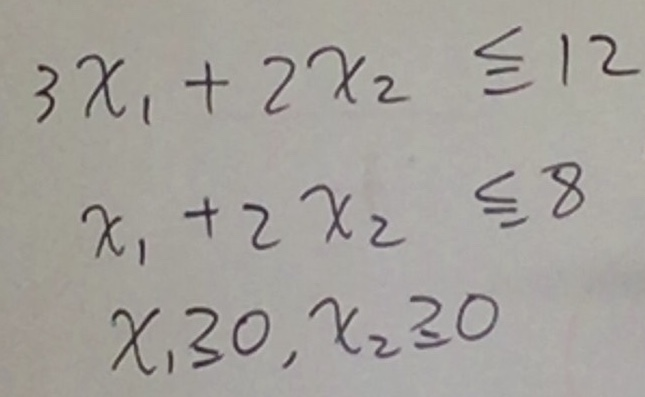
\includegraphics[width=7cm]{12_17_1.JPG}
\end{center}
\begin{enumerate}
\item 制約条件を図示する
	\begin{center}
		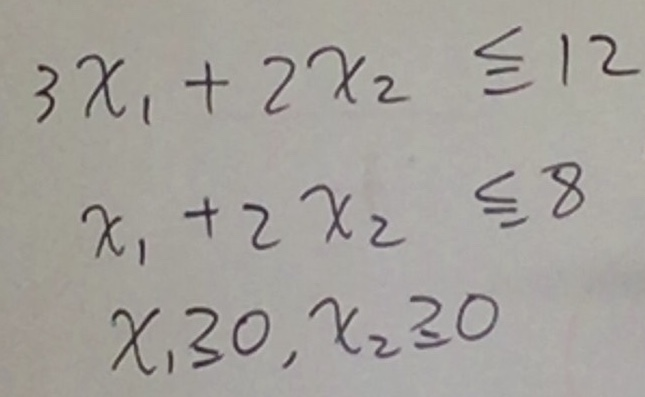
\includegraphics[width=7cm]{12_17_1.JPG}
	\end{center}
	実行可能領域=制約条件を満たす解の範囲
\item 目的関数の”等高線”を引く\\
	ここでいう等高線とは同じ値になるところという意味\\
	\begin{center}
		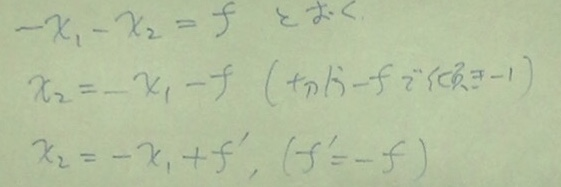
\includegraphics[width=7cm]{12_17_3.JPG}
	\end{center}
	\begin{center}
		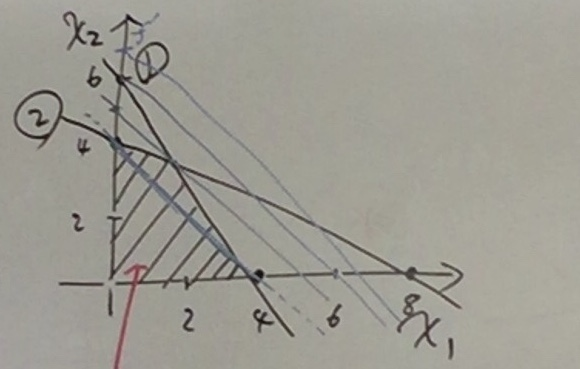
\includegraphics[width=7cm]{12_17_4.JPG}
	\end{center}

\item 最小化→fを小さくする=f'を大きくする\\
	1と2の交点を通るとき最大\\
	実行可能領域の凸多角形の頂点のうち、少なくとも1点は\textcolor{red}{最適解}になっている。\\
	↓\\
	n変数の場合も、空間${\bf{R}}^n$の凸面体の頂点が必ず最適解のになっている\\
	\\
	頂点だけ調べればいい||\\
	頂点の数は、nが大きくなると急激に増加する\\
\end{enumerate}
\subsection{シンプレックス法}
nが大きくなると関数ではしんどい\\
{\Large{シンプレックス法}}\\
実行可能領域の1つの頂点から初めて、目的関数の値が必ず減少するように、隣接する頂点に移動すれば、最終的に最適化に到達する。
	\subsubsection{例題(標準形を考える}
	目的関数:$-x_1-x_2→最小$
	制約関数:
	\begin{center}
		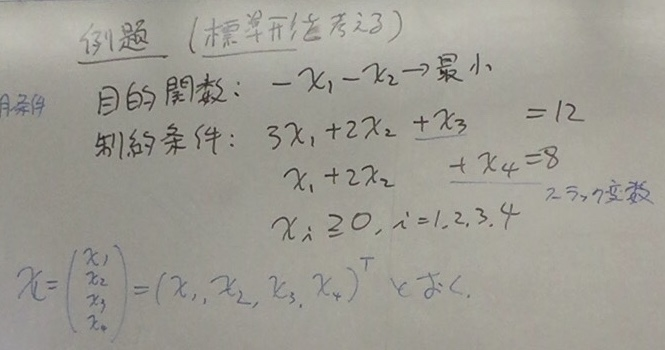
\includegraphics[width=7cm]{12_17_5.JPG}
	\end{center}
	{\large{変数の数は4つに対して、式が2つしかないので、普通にとくと解が出ない\\
	等式の制約条件は2つなので、4変数のうち2変数を0とおけば、残りの変数の値は一意に定まる。
	これを\textcolor{red}{基底解}と呼ぶ。\\
	基底解のうち、非負条件$\bf{x}≧\bf{0}$を満たすものを、\textcolor{red}{実行可能基底解とよぶ}}}\\
	\begin{description}
		\item [1. 初期条件]
			頂点(実行可能基底)を1つ求める。(a)〜(f)が基底解
			\begin{center}
				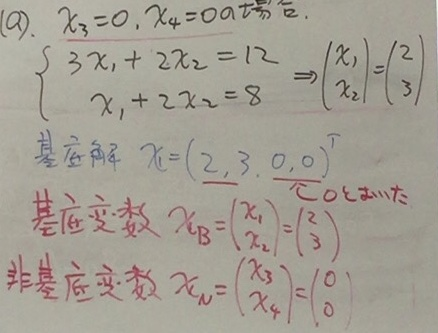
\includegraphics[width=7cm]{12_17_6.JPG}
			\end{center}
			\begin{center}
				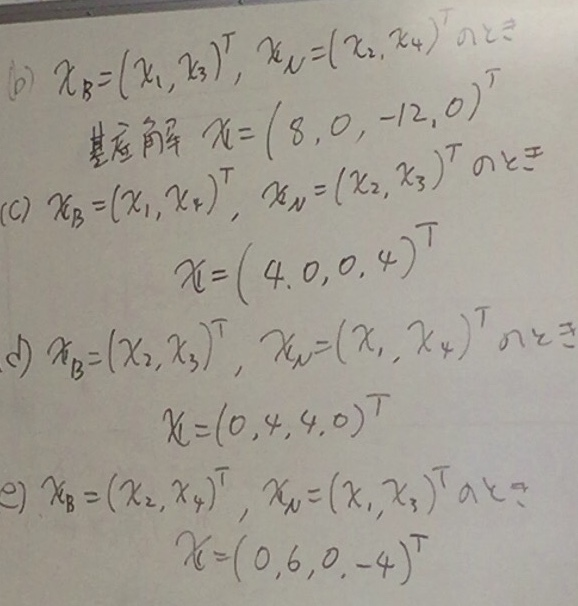
\includegraphics[width=7cm]{12_17_7.JPG}
			\end{center}
			\begin{center}
				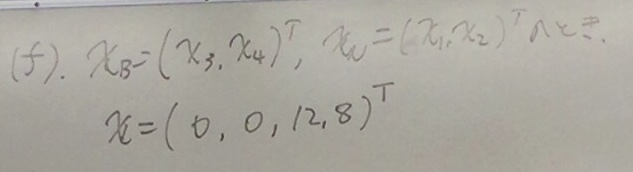
\includegraphics[width=7cm]{12_17_8.JPG}
			\end{center}
			\begin{center}
				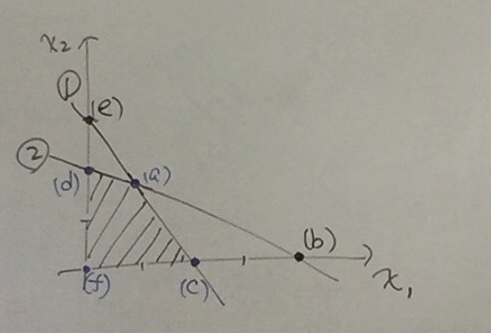
\includegraphics[width=7cm]{12_17_9.JPG}
			\end{center}
			知りたいのは実行可能基底解\\
			実行可能基底解は$\bf{x}≧\bf{0}$より、(a),(c),(d),(f)となる\\
			(b)と(e)は基底解だが、実行可能基底解ではない。\\
			
			{\large{行列とベクトルによる解放}}\\
			\begin{center}
				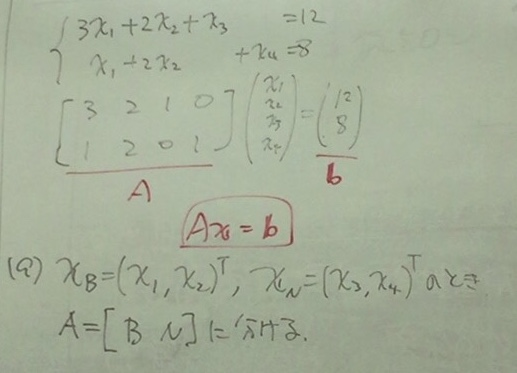
\includegraphics[width=7cm]{12_17_10.JPG}
			\end{center}
			\begin{center}
				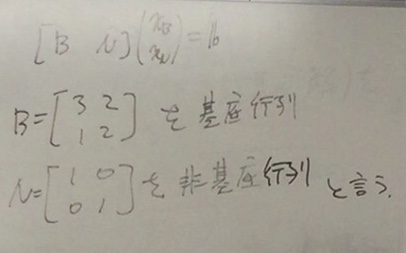
\includegraphics[width=7cm]{12_17_11.JPG}
			\end{center}	xt
			\begin{center}
				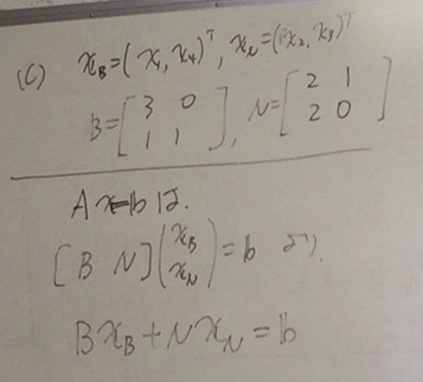
\includegraphics[width=7cm]{12_17_12.JPG}
			\end{center}
			\begin{center}
				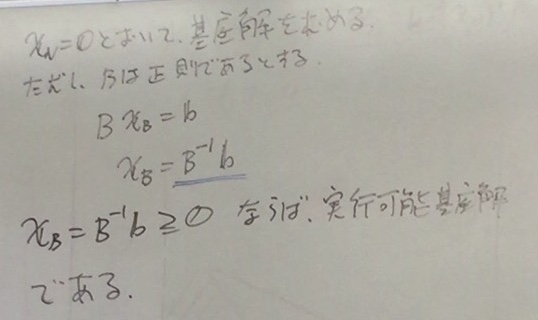
\includegraphics[width=7cm]{12_17_13.JPG}
			\end{center}
			↓\\
			凸多面体の頂点
		\item [2. 隣接する頂点に移動する]
			基底変数の1つと非基底変数の1つを交換する\\
			\begin{center}
				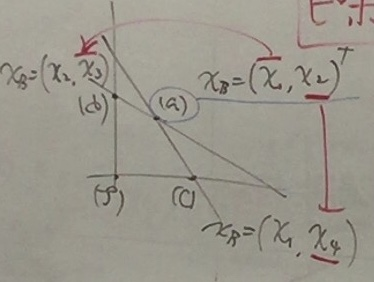
\includegraphics[width=7cm]{12_17_14.JPG}
			\end{center}
			↓\\
			\textcolor{red}{\large{ピボット操作}}という\\
			ピボット操作を繰り返して、実行可能基底解を次々に調べていくと、最適解にたどり着く
	\end{description}
	
\section{1/7}
\subsection{シンプレックス法の初期化}
初期化実行可能基底解を見つけるには、どのようにすれば良いか\\
{\textcolor{blue}{\Large{2段階法(2段階シンプレックス法)}}\\
初期実行可能基底解を求めるのに、さらにシンプレックス法を用いる方法\\
\subsubsection{例題}
	\begin{center}
		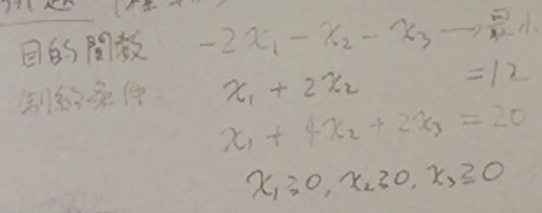
\includegraphics[width=7cm]{1_7_1.JPG}
	\end{center}
	\begin{center}
		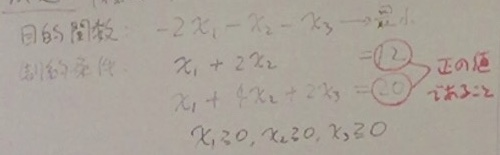
\includegraphics[width=7cm]{1_7_2.JPG}
	\end{center}
	初期実行基底解を求めるために、\textcolor{blue}{補助問題を考える}\\
	{\textcolor{blue}{\Large{補助問題}}}\\
	\begin{center}
		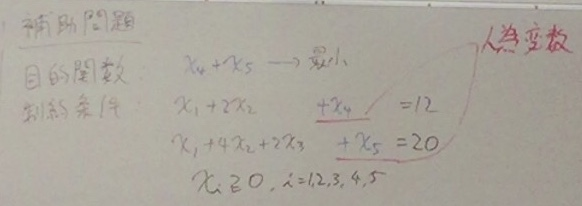
\includegraphics[width=7cm]{1_7_3.JPG}
	\end{center}
	************人為変数と前に使ったスラック変数の違い大事!!穴埋めでテストに出る !!\\
	補助問題の最小値が$0$ならば、$x_4=0.x_5=0$である。$x_1,x_2,x_3$はもとのの問題の制約条件を満たすので、実行可能解を与える\\
	補助問題の最小値が0である\\
	\[↓\]
	元の問題に実行可能解が存在する\\
	\textcolor{blue}{※最小値が0出ない場合、元の問題に最適解が存在しない}\\
	\begin{description}
		\item[第一段階]:補助問題をシンプレックス法で解き、元の問題の実行可能基底解をもとめる
		\item[第二段階]:元の問題をシンプレックス法で解く
	\end{description}
	補助問題をシンプレックス・タブローでとく。一番上の行が目的関数となるよー
	\begin{center}
		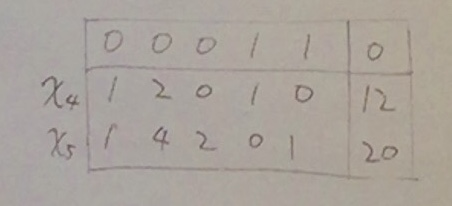
\includegraphics[width=7cm]{1_7_4.JPG}
	\end{center}
	基底変数として、人為変数の$x_4,x_5$を選ぶ。しかし、スラック変数と違って、上の段の$x_4,x_5$の係数が0になっていない\\
	\begin{center}
		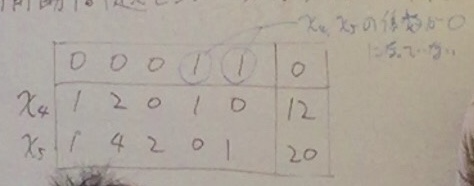
\includegraphics[width=7cm]{1_7_5.JPG}
	\end{center}
	→修正が必要\\
	基底変数$x_4,x_5$の係数が0になるように、行の演算をする\\
	・1行目から2行目と3行目の和を引くと、1行目の$x_4,x_5$の係数の値が0になる
	\begin{center}
		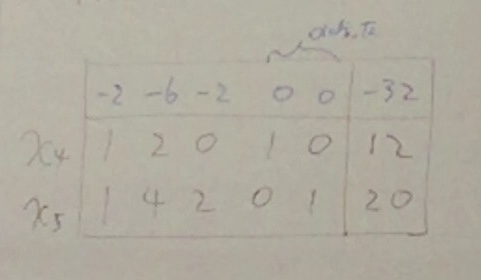
\includegraphics[width=7cm]{1_7_6.JPG}
	\end{center}
	これによりシンプレックス・タブローで解くことができる\\
	1行目で一番小さいやつをピボット列とする。一番左の値をピボット列でそれぞれ割って、小さい方をピボット値とする\\
	\begin{center}
		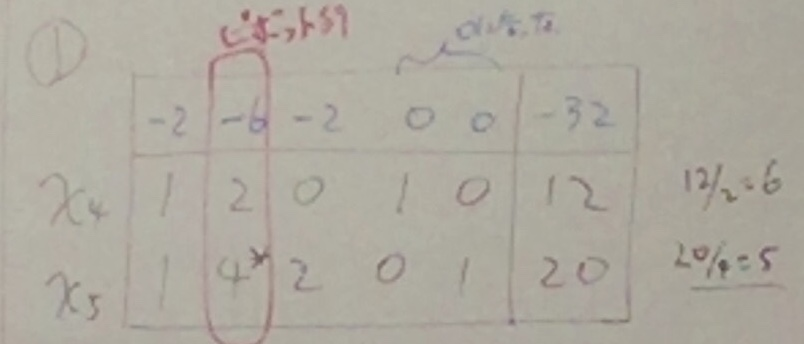
\includegraphics[width=7cm]{1_7_7.JPG}
	\end{center}
	0になるように1行目2行目を計算,1行目で小さいやつをピポット列
	\begin{center}
		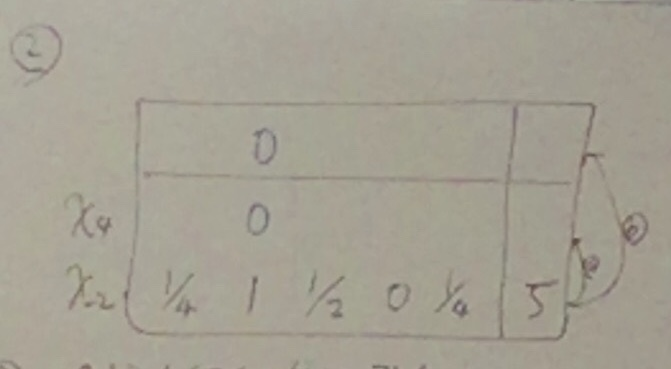
\includegraphics[width=7cm]{1_7_8.JPG}
	\end{center}
	\begin{center}
		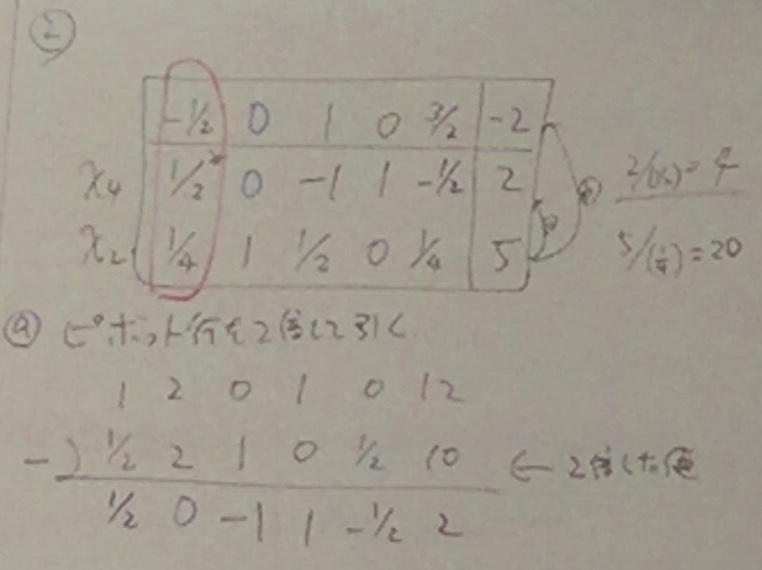
\includegraphics[width=7cm]{1_7_9.JPG}
	\end{center}
	\begin{center}
		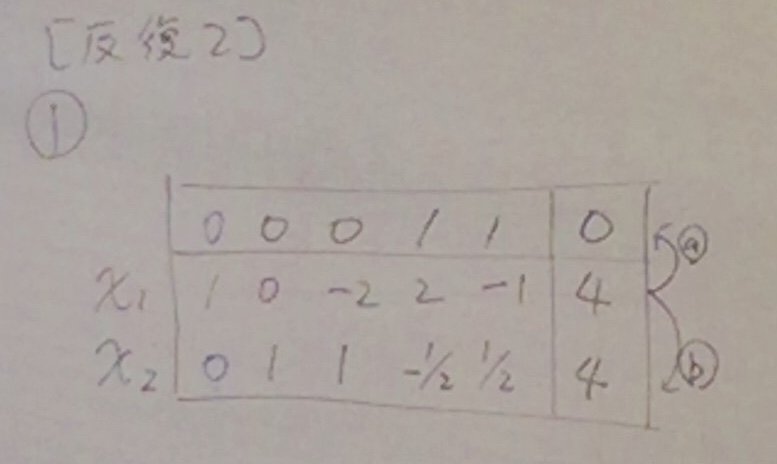
\includegraphics[width=7cm]{1_7_10.JPG}
	\end{center}
	1行目がすべて0以上になったので終了\\
	一番左の$x_1,x_2$が基底変数、その他の変数は非基底変数\\
	これらの違いは基底変数は解、非基底変数は0となるよって\\
	最適解は
	\begin{center}
		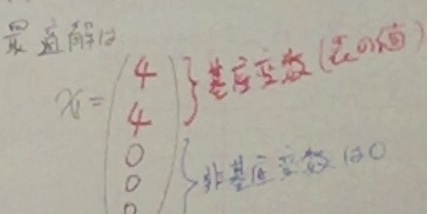
\includegraphics[width=7cm]{1_7_11.JPG}
	\end{center}
	であり、この時の最適値(目的関数の値)は0になる。一番左上のマイナスの値(今回は0なので-0)\\
	・人為変数$x_4,x_5$の値は0であり、最小値0となっている。\\
	{\Large{●第二段階}}\\
	第一段階の結果より
	\begin{center}
		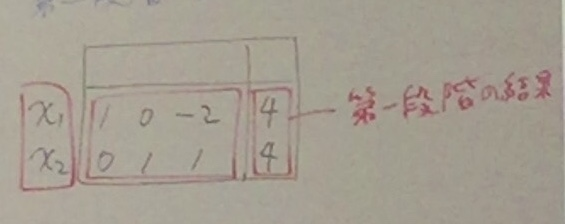
\includegraphics[width=7cm]{1_7_12.JPG}
	\end{center}
	元の目的関数の係数を1行目に書く
	\begin{center}
		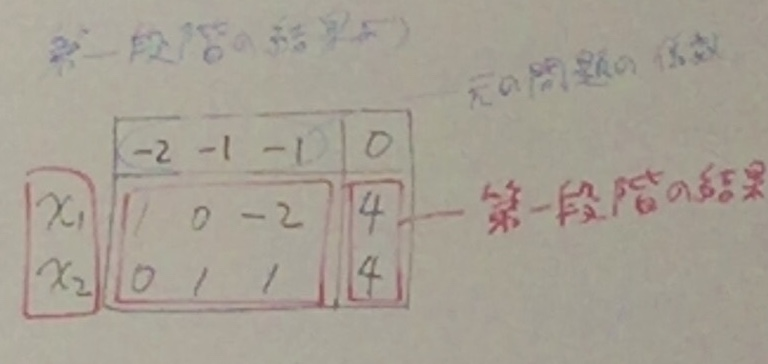
\includegraphics[width=7cm]{1_7_13.JPG}
	\end{center}
	基底変数$x_1,x_2$の係数が0になっていないので、行操作を行い0にする。\\
	●2行目を2倍したものと、3行目の和を1行目に足す\\
	\begin{center}
		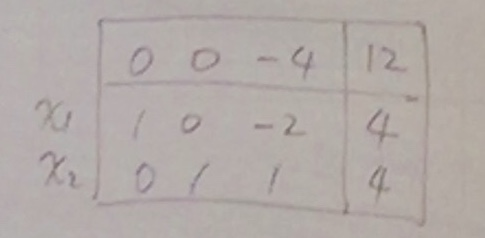
\includegraphics[width=7cm]{1_7_14.JPG}
	\end{center}
	ビボットを求める。負の方は除外するので自動的に3列目の1がピボット。
	\begin{center}
		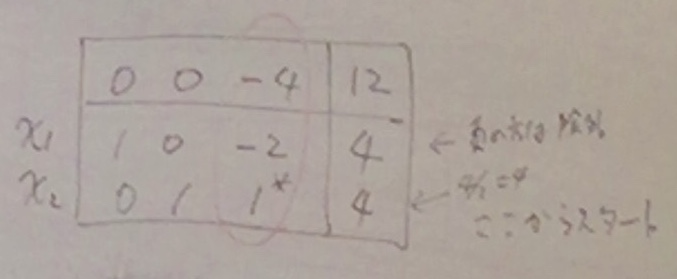
\includegraphics[width=7cm]{1_7_15.JPG}
	\end{center}
	\begin{center}
		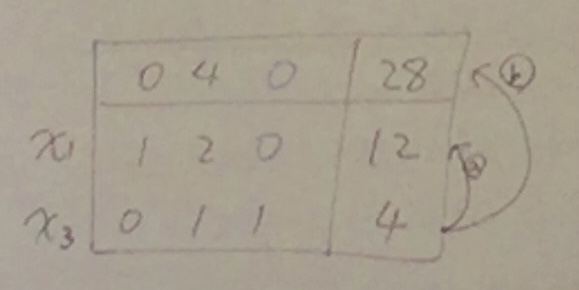
\includegraphics[width=7cm]{1_7_16.JPG}
	\end{center}
	1行目に負の値がないので終了。\\
	最適解は
	\begin{center}
		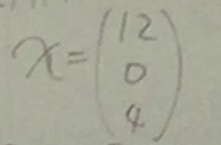
\includegraphics[width=7cm]{1_7_17.JPG}
	\end{center}
	であり、この時の最適値は、-28になる(マイナスを忘れないように)

\section{1/21}
	テスト範囲2-7まで\\
	シンプレックスタブローの解き方は覚える\\
	2段階法は初期値がわからん時に使う\\
	標準形になおすことが大事!!\\
	線形代数の問題がでるよ$\bf{x}^T\bf{y}=$とか
	\subsection{双対法}
		与えられた任意の線形計画問題(主問題)に対して、その双対問題と呼ばれる、もう1つの線型計画法が存在する。\\
		標準形の問題\\
		目的関数:$\bf{C}^T\bf{x} → 最小$\\
		制約条件:$A\bf{x}=\bf{b} , \bf{x}≧\bf{0}$\\
		これを主問題とすると、双対問題は\\
		目的関数:$\bf{b}^T\bf{w} → 最小$\\
		制約条件:$A^T\bf{w}≦\bf{C}$\\
		と定義される。(定義なのでこういうもの)\\
		**例題\\
		目的関数:$\bf{C}^T\bf{x} → 最小$\\
		制約条件:$A\bf{x}≧\bf{b},\bf{x}≧\bf{0}$\\
		この問題の双対問題を求めなさい。\\
		\begin{enumerate}
			\item 標準形にする
				\begin{center}
					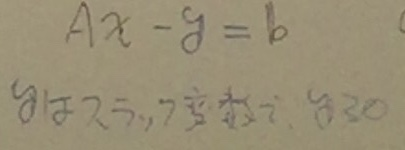
\includegraphics[width=7cm]{1_21_2.JPG}
				\end{center}
				\begin{center}
					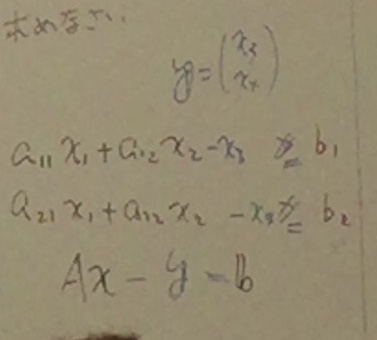
\includegraphics[width=7cm]{1_21_1.JPG}
				\end{center}
				\begin{center}
					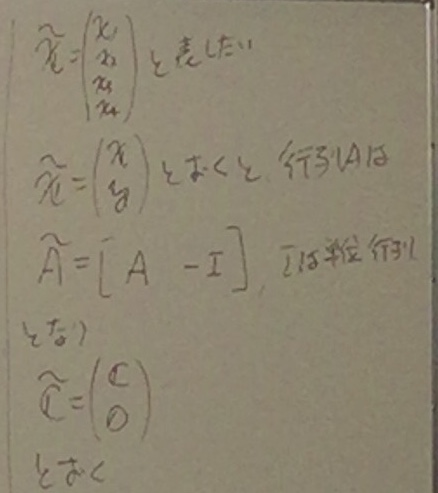
\includegraphics[width=7cm]{1_21_3.JPG}
				\end{center}
				\begin{center}
					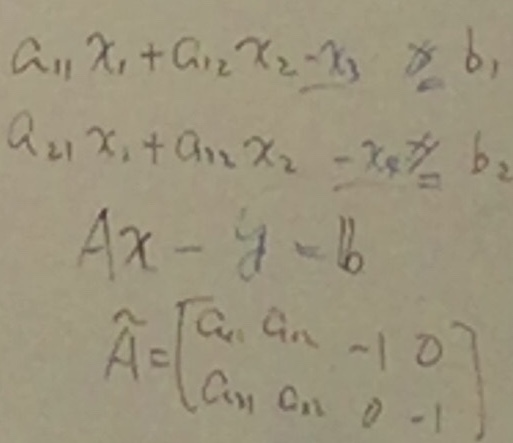
\includegraphics[width=7cm]{1_21_4.JPG}
				\end{center}
				このように変数を置き換えると\\
				\begin{center}
					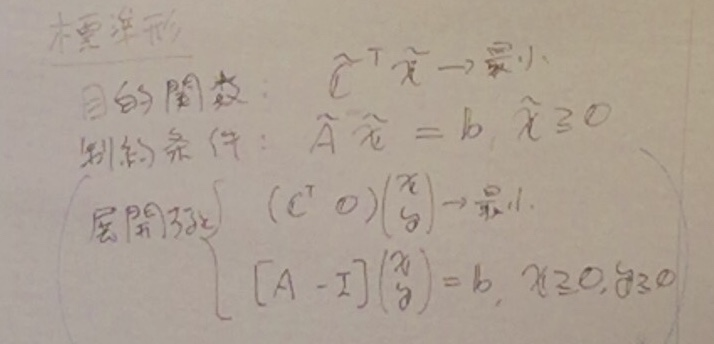
\includegraphics[width=7cm]{1_21_5.JPG}
				\end{center}
			\item 双対問題にする\\
				\begin{center}
					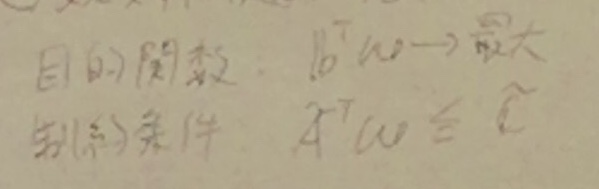
\includegraphics[width=7cm]{1_21_6.JPG}
				\end{center}	
				\item 置いたやつをもとにもどす\\
				\begin{center}
					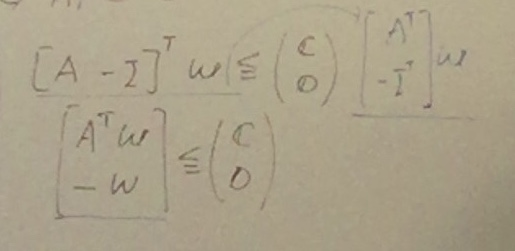
\includegraphics[width=7cm]{1_21_7.JPG}
				\end{center}	
				\begin{center}
					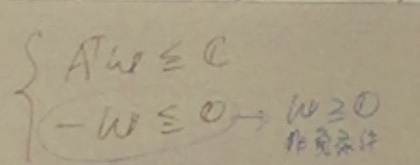
\includegraphics[width=7cm]{1_21_8.JPG}
				\end{center}	
		\end{enumerate}
		これより、双対問題は
		\begin{center}
			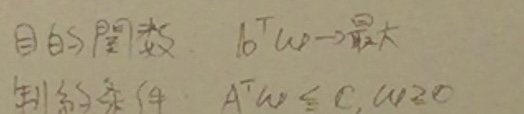
\includegraphics[width=7cm]{1_21_9.JPG}
		\end{center}	
		となる。
		\subsection{双対問題}
			"双対問題"を主問題とみなすと、元の"主問題"が双対問題となる。\\
			主問題を(P)\\
			双対問題を(D)で表す\\
		\subsection{弱双対定理}
			(P)と(D)のそれぞれの任意の実行可能解$\bf{x}$と$\bf{w}$に対して、常に不等式
			\[
				\bf{C}^T≧\bf{b}^T\bf{w}
			\]
			が成り立つ\\
			(証明)\\
			(P)の制約条件$A\bf{x}=\bf{b},\bf{x}≧\bf{0}$と(D)の制約条件$A\bf{w}≦\bf{C}$より
			\begin{center}
				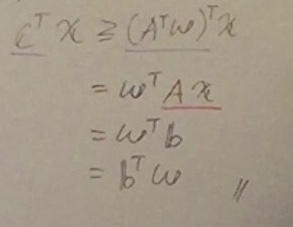
\includegraphics[width=7cm]{1_21_10.JPG}
			\end{center}
			→\textcolor{red}{テスト出るかも}\\
			\begin{itemize}
				\item (P)の任意の実行可能解$\bf{x}$に対して
				\[
					\bf{C}^T\bf{x}≧(D)の最大値
				\]
				が成り立つ。また、(D)の任意の実行可能解$\bf{w}$に対して、
				\[
					(P)の最小値≧\bf{b}^T\bf{w}
				\]
				が成り立つ。\\
				\item (P)と(D)のそれぞれの実行可能解$\bf{x},\bf{w}$が
				\[
					\bf{C}^T\bf{x}=\bf{b}^T\bf{w}
				\]
				を満たせば、$\bf{x}$と$\bf{w}$はそれぞれの最適解である。\\
				\item (P)が有界でないならば、(D)は実行可能解を持たない。\\
					また、(D)が有界でないならば、(P)は実行可能解を持たない\\
			\end{itemize}
			(P)の最小値を求めることが、難しいならば、(D)の実行可能解$\bf{w}$を1つ見つけて、$\bf{b}^T\bf{w}$を求めることで、(P)の最小値の下限を知ることができる。
		\subsection{双対定理}
			(P)または(D)の一方が最適解を持つならば、他方も最適解を持ち、(P)の最小値と(D)の最大値は一致する\\
			(証明)\\
			標準形の主問題(P)が最適解$\bf{x}*$をもつとすると
			\[
				\bf{x}_B*=B^{-1}\bf{b},\bf{x}_N*=\bf{0}
			\]
			ただし、$A=[B N]$とする。\\
			ここで、(D)のベクトル$\bf{w}*$を\bf{w}*=(B^{-1})^T\bf{C}_B$と定義する。\\
			これより、
			\[
				B^T\bf{w}*=\bf{C}_B
			\]
			となる\\
			相対コスト係数\\
			\[
				\bf{C}_N^T-C_B^TB^{-1}N≧\bf{0}
			\]
			より
			\begin{center}
				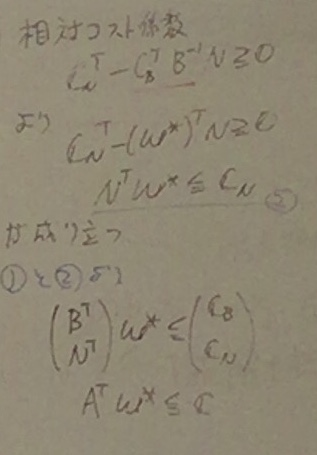
\includegraphics[width=7cm]{1_21_11.JPG}
			\end{center}
			よって、$\bf{w}*$は(D)の制約条件を満たす\\
			つまり、実行可能解である。\\
			さらに
			\begin{center}
				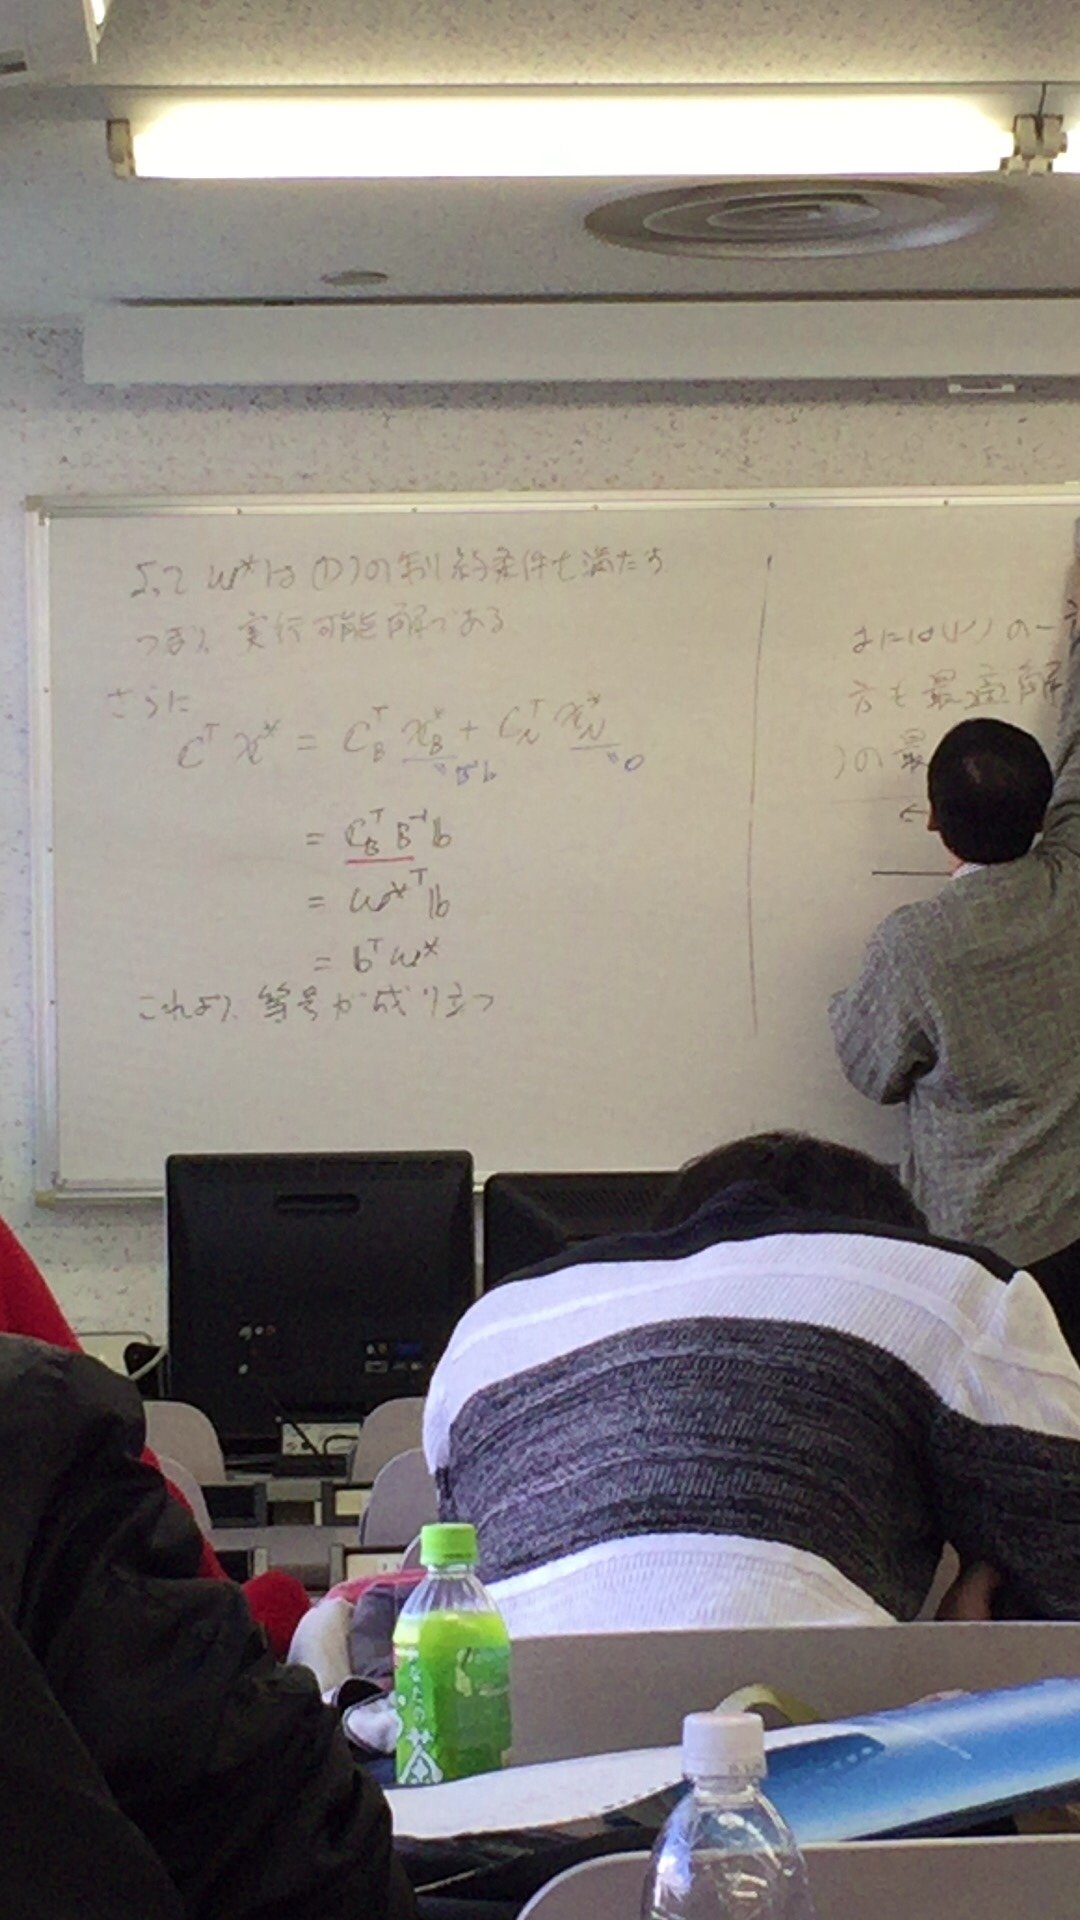
\includegraphics[width=7cm]{1_21_12.JPG}
			\end{center}
			これにより、冬瓜雨が成り立つ。\\
			以上より、弱双対定理の2より、$\bf{w}*$は(D)の最適解である。\\
			また、(P)の最小値は(D)の最大値と等しい。\\
			系;(P)と(D)がともに実行可能解を持てば、それらは最適解をもつ\\
			(P)の最小値と(D)の最小値は等しい\\
			
\end{document}













